\documentclass{standalone}
\usepackage{tikz}
\usetikzlibrary{patterns, positioning}


\begin{document}
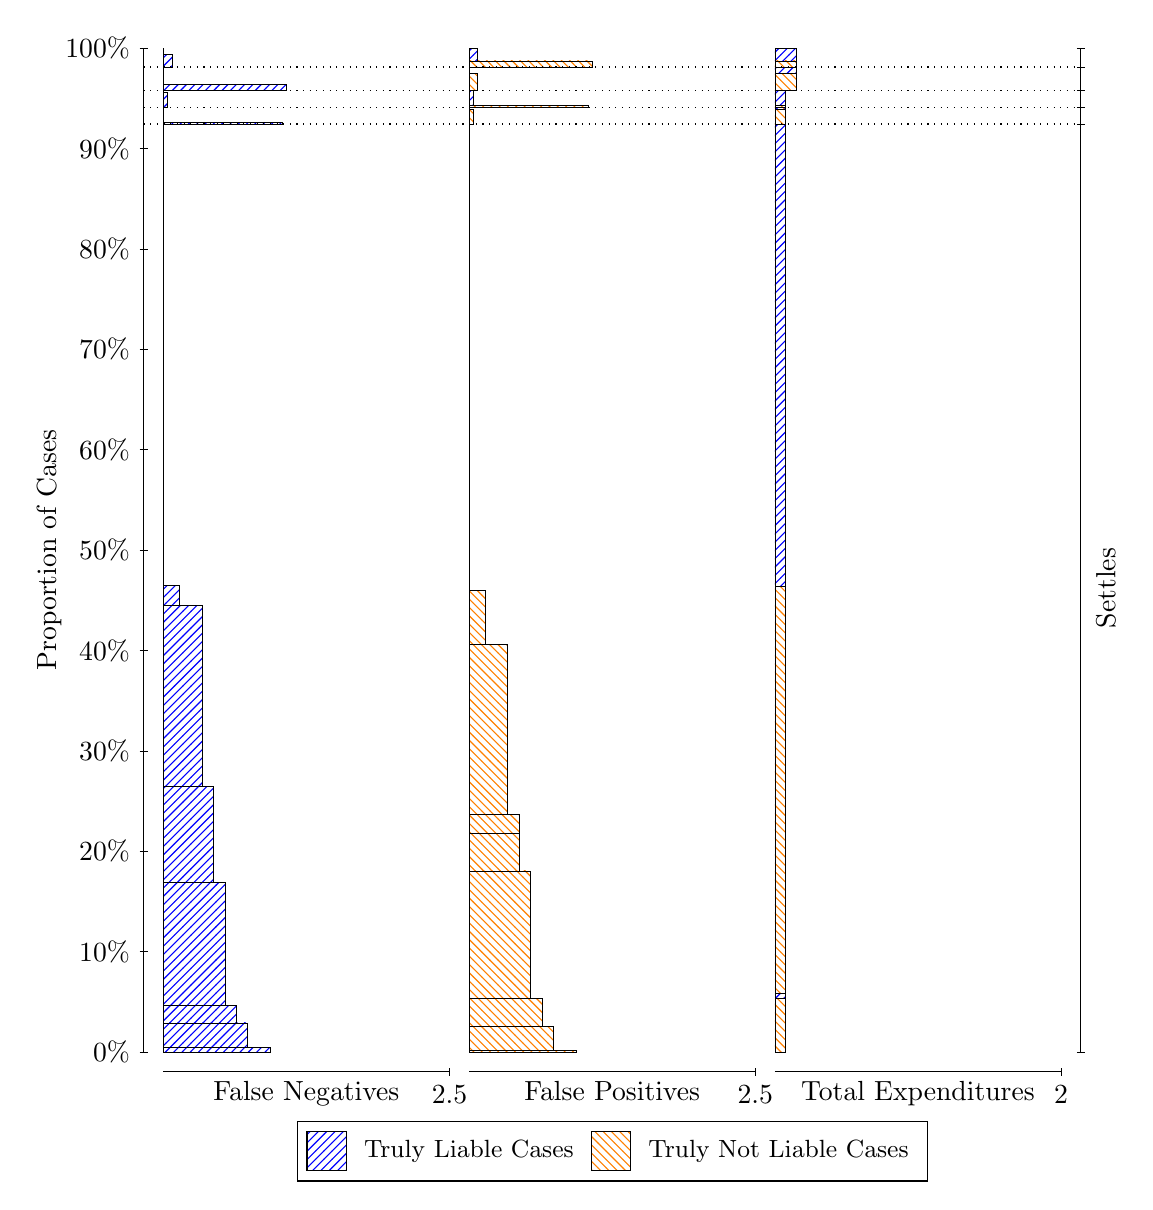
\begin{tikzpicture}
\draw[black, very thin] (1.5,1.75) -- (1.5,14.5);
\node[rotate=90, text=black, anchor=center] at (0.3, 8.125) {Proportion of Cases};
\draw[black, very thin] (1.45,1.75) -- (1.55,1.75);
\node[text=black, anchor=east] at (1.45, 1.75) {0\%};
\draw[black, very thin] (1.45,3.025) -- (1.55,3.025);
\node[text=black, anchor=east] at (1.45, 3.025) {10\%};
\draw[black, very thin] (1.45,4.3) -- (1.55,4.3);
\node[text=black, anchor=east] at (1.45, 4.3) {20\%};
\draw[black, very thin] (1.45,5.575) -- (1.55,5.575);
\node[text=black, anchor=east] at (1.45, 5.575) {30\%};
\draw[black, very thin] (1.45,6.85) -- (1.55,6.85);
\node[text=black, anchor=east] at (1.45, 6.85) {40\%};
\draw[black, very thin] (1.45,8.125) -- (1.55,8.125);
\node[text=black, anchor=east] at (1.45, 8.125) {50\%};
\draw[black, very thin] (1.45,9.4) -- (1.55,9.4);
\node[text=black, anchor=east] at (1.45, 9.4) {60\%};
\draw[black, very thin] (1.45,10.675) -- (1.55,10.675);
\node[text=black, anchor=east] at (1.45, 10.675) {70\%};
\draw[black, very thin] (1.45,11.95) -- (1.55,11.95);
\node[text=black, anchor=east] at (1.45, 11.95) {80\%};
\draw[black, very thin] (1.45,13.225) -- (1.55,13.225);
\node[text=black, anchor=east] at (1.45, 13.225) {90\%};
\draw[black, very thin] (1.45,14.5) -- (1.55,14.5);
\node[text=black, anchor=east] at (1.45, 14.5) {100\%};

\draw[black, very thin] (13.4,1.75) -- (13.4,14.5);
\draw[black, very thin] (13.35,1.75) -- (13.45,1.75);
\node[anchor=west] at (13.35, 1.75) {};
\draw[black, very thin] (13.35,13.535) -- (13.45,13.535);
\node[anchor=west] at (13.35, 13.535) {};
\draw[black, very thin] (13.35,13.747) -- (13.45,13.747);
\node[anchor=west] at (13.35, 13.747) {};
\draw[black, very thin] (13.35,13.959) -- (13.45,13.959);
\node[anchor=west] at (13.35, 13.959) {};
\draw[black, very thin] (13.35,14.259) -- (13.45,14.259);
\node[anchor=west] at (13.35, 14.259) {};
\draw[black, very thin] (13.35,14.5) -- (13.45,14.5);
\node[anchor=west] at (13.35, 14.5) {};

\draw[black, very thin, pattern color=blue, pattern=north east lines] (1.75,1.75) rectangle (3.1125,1.8042);
\draw[black, very thin, pattern color=blue, pattern=north east lines] (1.75,1.8042) rectangle (2.8218,2.1192);
\draw[black, very thin, pattern color=blue, pattern=north east lines] (1.75,2.1192) rectangle (2.6765,2.3465);
\draw[black, very thin, pattern color=blue, pattern=north east lines] (1.75,2.3465) rectangle (2.5312,3.906);
\draw[black, very thin, pattern color=blue, pattern=north east lines] (1.75,3.906) rectangle (2.3858,5.1264);
\draw[black, very thin, pattern color=blue, pattern=north east lines] (1.75,5.1264) rectangle (2.2405,7.4245);
\draw[black, very thin, pattern color=blue, pattern=north east lines] (1.75,7.4245) rectangle (1.9498,7.6715);
\draw[black, very thin, pattern color=orange, pattern=north west lines] (1.75,7.6715) rectangle (1.75,13.535);
\draw[black, very thin, pattern color=blue, pattern=north east lines] (1.75,13.535) rectangle (3.2578,13.555);
\draw[black, very thin, pattern color=orange, pattern=north west lines] (1.75,13.555) rectangle (1.75,13.747);
\draw[black, very thin, pattern color=blue, pattern=north east lines] (1.75,13.747) rectangle (1.8045,13.939);
\draw[black, very thin, pattern color=orange, pattern=north west lines] (1.75,13.939) rectangle (1.75,13.959);
\draw[black, very thin, pattern color=blue, pattern=north east lines] (1.75,13.959) rectangle (3.3123,14.036);
\draw[black, very thin, pattern color=orange, pattern=north west lines] (1.75,14.036) rectangle (1.75,14.259);
\draw[black, very thin, pattern color=blue, pattern=north east lines] (1.75,14.259) rectangle (1.859,14.423);
\draw[black, very thin, pattern color=orange, pattern=north west lines] (1.75,14.423) rectangle (1.75,14.5);
\draw[black, very thin, pattern color=orange, pattern=north west lines] (5.6333,1.75) rectangle (6.9958,1.7668);
\draw[black, very thin, pattern color=orange, pattern=north west lines] (5.6333,1.7668) rectangle (6.7052,2.075);
\draw[black, very thin, pattern color=orange, pattern=north west lines] (5.6333,2.075) rectangle (6.5598,2.4346);
\draw[black, very thin, pattern color=orange, pattern=north west lines] (5.6333,2.4346) rectangle (6.4145,4.0498);
\draw[black, very thin, pattern color=orange, pattern=north west lines] (5.6333,4.0498) rectangle (6.2692,4.529);
\draw[black, very thin, pattern color=orange, pattern=north west lines] (5.6333,4.529) rectangle (6.2692,4.7646);
\draw[black, very thin, pattern color=orange, pattern=north west lines] (5.6333,4.7646) rectangle (6.1238,6.9276);
\draw[black, very thin, pattern color=orange, pattern=north west lines] (5.6333,6.9276) rectangle (5.8332,7.6132);
\draw[black, very thin, pattern color=blue, pattern=north east lines] (5.6333,7.6132) rectangle (5.6333,13.535);
\draw[black, very thin, pattern color=orange, pattern=north west lines] (5.6333,13.535) rectangle (5.6878,13.726);
\draw[black, very thin, pattern color=blue, pattern=north east lines] (5.6333,13.726) rectangle (5.6333,13.747);
\draw[black, very thin, pattern color=orange, pattern=north west lines] (5.6333,13.747) rectangle (7.1412,13.768);
\draw[black, very thin, pattern color=blue, pattern=north east lines] (5.6333,13.768) rectangle (5.6878,13.959);
\draw[black, very thin, pattern color=orange, pattern=north west lines] (5.6333,13.959) rectangle (5.7423,14.182);
\draw[black, very thin, pattern color=blue, pattern=north east lines] (5.6333,14.182) rectangle (5.6333,14.259);
\draw[black, very thin, pattern color=orange, pattern=north west lines] (5.6333,14.259) rectangle (7.1957,14.336);
\draw[black, very thin, pattern color=blue, pattern=north east lines] (5.6333,14.336) rectangle (5.7423,14.5);
\draw[black, very thin, pattern color=orange, pattern=north west lines] (9.5167,1.75) rectangle (9.6529,2.4356);
\draw[black, very thin, pattern color=blue, pattern=north east lines] (9.5167,2.4356) rectangle (9.6529,2.4898);
\draw[black, very thin, pattern color=orange, pattern=north west lines] (9.5167,2.4898) rectangle (9.6529,7.6675);
\draw[black, very thin, pattern color=blue, pattern=north east lines] (9.5167,7.6675) rectangle (9.6529,13.535);
\draw[black, very thin, pattern color=orange, pattern=north west lines] (9.5167,13.535) rectangle (9.6529,13.726);
\draw[black, very thin, pattern color=blue, pattern=north east lines] (9.5167,13.726) rectangle (9.6529,13.747);
\draw[black, very thin, pattern color=orange, pattern=north west lines] (9.5167,13.747) rectangle (9.6529,13.768);
\draw[black, very thin, pattern color=blue, pattern=north east lines] (9.5167,13.768) rectangle (9.6529,13.959);
\draw[black, very thin, pattern color=orange, pattern=north west lines] (9.5167,13.959) rectangle (9.7892,14.182);
\draw[black, very thin, pattern color=blue, pattern=north east lines] (9.5167,14.182) rectangle (9.7892,14.259);
\draw[black, very thin, pattern color=orange, pattern=north west lines] (9.5167,14.259) rectangle (9.7892,14.336);
\draw[black, very thin, pattern color=blue, pattern=north east lines] (9.5167,14.336) rectangle (9.7892,14.5);
\draw[black, dotted] (1.5,13.535) -- (13.4,13.535);
\draw[black, dotted] (1.5,13.747) -- (13.4,13.747);
\draw[black, dotted] (1.5,13.959) -- (13.4,13.959);
\draw[black, dotted] (1.5,14.259) -- (13.4,14.259);
\draw[black, very thin] (1.75,1.5) -- (5.3833,1.5);
\node[text=black, anchor=north] at (3.5667, 1.5) {False Negatives};
\draw[black, very thin] (5.3833,1.45) -- (5.3833,1.55);
\node[text=black, anchor=north] at (5.3833, 1.45) {2.5};

\draw[black, very thin] (5.6333,1.5) -- (9.2667,1.5);
\node[text=black, anchor=north] at (7.45, 1.5) {False Positives};
\draw[black, very thin] (9.2667,1.45) -- (9.2667,1.55);
\node[text=black, anchor=north] at (9.2667, 1.45) {2.5};

\draw[black, very thin] (9.5167,1.5) -- (13.15,1.5);
\node[text=black, anchor=north] at (11.333, 1.5) {Total Expenditures};
\draw[black, very thin] (13.15,1.45) -- (13.15,1.55);
\node[text=black, anchor=north] at (13.15, 1.45) {2};

\node[text=black, centered, rotate=90] at (13.72, 7.6424) {Settles};





\draw (7.449999999999999,1.5) node[draw=none] (baseCoordinate) {};
\begin{scope}[align=center]
        \matrix[scale=0.5, draw=black, below=0.5cm of baseCoordinate, nodes={draw}, column sep=0.1cm]{
            \node[rectangle, draw, minimum width=0.5cm, minimum height=0.5cm, pattern color=blue, pattern=north east lines] {}; &
            \node[draw=none, font=\small, text=black] (B) {Truly Liable Cases}; &
            \node[rectangle, draw, minimum width=0.5cm, minimum height=0.5cm, pattern color=orange, pattern=north west lines] {}; &
            \node[draw=none, font=\small, text=black] (B) {Truly Not Liable Cases}; \\
            };
\end{scope}

\end{tikzpicture}
\end{document}